\testfile{pgfplotstest.hansmeine\_app.tex}
\testsection{Application example of Hans Meine}
\begingroup
This example has been copied with permission from 

\noindent
\url{http://kogs-www.informatik.uni-hamburg.de/~meine/tikz/plots}.

Please note that the first plot's input data as it is found in the url above is slightly shifted compared to the other plots.

\tikzstyle{plot legend}=[
   rounded corners=2.5pt,inner xsep=3pt,inner ysep=2pt,
   draw=black!50,fill=white,
   font=\footnotesize,cells={anchor=center},
   nodes={inner sep=2pt,text depth=0.15em,rounded corners=0pt,right}]

\tikzstyle{every axis legend}=[plot legend,at={(.85,0.8)},below right]
\tikzstyle{every axis y label}=[at={(0,0.5)},xshift=-25pt,rotate=90]

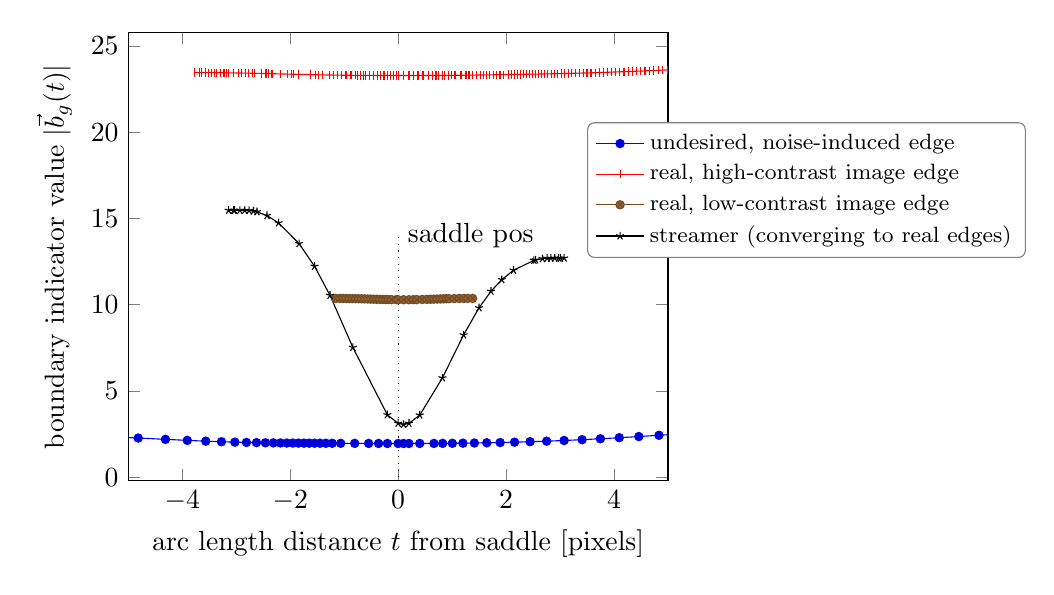
\begin{tikzpicture}[mark size=1.5pt,remember picture]

\begin{axis}[
  xmin=-5,xmax=5,
  %ymin=0,ymax=25,
  %ytick={0,5,...,25},
  xlabel={arc length distance $t$ from saddle [pixels]},
  ylabel={boundary indicator value $|\vec{b}_g(t)|$}]

\addplot plot coordinates {
  (-6.74792,2.41861) (-6.66786,2.41852) (-6.58805,2.41824) (-6.50996,2.41777) (-6.41075,2.41679) (-6.30551,2.41505) (-6.15340,2.41075) (-5.93965,2.40070) (-5.62466,2.37734) (-5.15092,2.32533) (-4.81777,2.27973) (-4.31289,2.20389) (-3.90792,2.14396) (-3.56562,2.09832) (-3.27459,2.06512) (-3.02640,2.04160) (-2.81205,2.02498) (-2.62515,2.01318) (-2.46036,2.00469) (-2.31403,1.99851) (-2.18241,1.99390) (-2.06229,1.99036) (-1.95106,1.98758) (-1.84645,1.98531) (-1.74609,1.98339) (-1.64791,1.98171) (-1.54947,1.98017) (-1.44841,1.97871) (-1.34122,1.97723) (-1.22126,1.97565) (-1.06446,1.97363) (-0.80552,1.97038) (-0.54659,1.96739) (-0.36271,1.96559) (-0.20000,1.96437) (0.00000,1.96349) (0.10000,1.96337) (0.20000,1.96350) (0.40000,1.96457) (0.66334,1.96786) (0.82469,1.97106) (1.00410,1.97577) (1.20014,1.98238) (1.41256,1.99137) (1.64222,2.00335) (1.88995,2.01902) (2.15698,2.03926) (2.44428,2.06507) (2.75132,2.09742) (3.07466,2.13693) (3.40793,2.18352) (3.74762,2.23692) (4.09685,2.29747) (4.45942,2.36533) (4.83307,2.43910) (5.20177,2.51426) (5.54872,2.58624) (5.87085,2.65390) (6.17726,2.71933) (6.47863,2.78542) (6.78862,2.85637) (7.13375,2.94064) (7.59098,3.06389) (8.13953,3.23189) (8.67260,3.41315) (9.39853,3.66690) (9.83987,3.80614) (10.13601,3.88485) (10.36232,3.93412) (10.54394,3.96577) (10.69550,3.98653) (10.83385,4.00111) (10.95513,4.01094) (11.03401,4.01619) (11.09168,4.01963) (11.14379,4.02251) (11.19194,4.02503) (11.28684,4.02965) (11.33618,4.03190) (11.38800,4.03416) (11.44303,4.03643) (11.50199,4.03872) (11.56561,4.04104) (11.63478,4.04335) (11.70991,4.04562) (11.79157,4.04779) (11.87873,4.04976) (11.96931,4.05140) (12.05829,4.05260) (12.14019,4.05335) (12.20972,4.05369) (12.26727,4.05379)
};
\addlegendentry{undesired, noise-induced edge}

\addplot[mark=|,red] plot coordinates {
  (-3.76974,23.44724) (-3.68200,23.44695) (-3.64029,23.44663) (-3.57390,23.44586) (-3.51311,23.44490) (-3.46300,23.44393) (-3.39804,23.44243) (-3.36070,23.44145) (-3.29129,23.43940) (-3.22822,23.43728) (-3.18614,23.43574) (-3.13754,23.43383) (-3.04637,23.42987) (-2.95967,23.42567) (-2.90068,23.42257) (-2.83380,23.41883) (-2.77416,23.41531) (-2.70061,23.41071) (-2.66154,23.40816) (-2.52857,23.39898) (-2.44938,23.39318) (-2.39931,23.38941) (-2.33883,23.38476) (-2.17413,23.37174) (-2.05644,23.36230) (-1.98196,23.35636) (-1.93330,23.35251) (-1.84825,23.34590) (-1.62954,23.32990) (-1.52996,23.32327) (-1.47585,23.31985) (-1.40329,23.31551) (-1.27105,23.30830) (-1.19944,23.30478) (-1.13051,23.30165) (-1.04894,23.29825) (-0.96702,23.29516) (-0.87382,23.29203) (-0.79070,23.28955) (-0.74927,23.28843) (-0.70129,23.28721) (-0.64637,23.28592) (-0.60115,23.28493) (-0.53219,23.28358) (-0.45855,23.28230) (-0.38244,23.28116) (-0.32153,23.28038) (-0.26284,23.27973) (-0.19690,23.27911) (-0.13978,23.27868) (-0.08064,23.27834) (-0.02275,23.27808) (0.00000,23.27801) (0.10000,23.27787) (0.20000,23.27802) (0.27601,23.27832) (0.36681,23.27891) (0.46110,23.27978) (0.55399,23.28091) (0.64198,23.28223) (0.70081,23.28326) (0.75328,23.28427) (0.81782,23.28563) (0.85871,23.28657) (0.93657,23.28849) (0.98295,23.28974) (1.05394,23.29177) (1.14949,23.29476) (1.16854,23.29539) (1.25761,23.29848) (1.31224,23.30049) (1.37408,23.30286) (1.44949,23.30589) (1.51818,23.30877) (1.57749,23.31135) (1.64391,23.31433) (1.69761,23.31680) (1.77152,23.32030) (1.82174,23.32272) (1.88683,23.32592) (1.95135,23.32914) (2.04539,23.33393) (2.09220,23.33636) (2.15071,23.33942) (2.21378,23.34276) (2.27209,23.34589) (2.32331,23.34867) (2.37362,23.35143) (2.42883,23.35450) (2.48828,23.35785) (2.54699,23.36122) (2.60335,23.36450) (2.65867,23.36780) (2.71561,23.37126) (2.77485,23.37495) (2.83543,23.37882) (2.89585,23.38280) (2.95675,23.38694) (3.01953,23.39134) (3.08437,23.39604) (3.15018,23.40099) (3.21683,23.40618) (3.28460,23.41165) (3.35451,23.41750) (3.42648,23.42374) (3.49957,23.43030) (3.57365,23.43717) (3.64867,23.44436) (3.72416,23.45181) (3.80056,23.45956) (3.87760,23.46758) (3.95468,23.47580) (4.03184,23.48421) (4.10882,23.49279) (4.18576,23.50154) (4.26266,23.51047) (4.33974,23.51959) (4.41715,23.52894) (4.49513,23.53857) (4.57441,23.54856) (4.65443,23.55888) (4.73544,23.56957) (4.81782,23.58073) (4.90189,23.59242) (4.98799,23.60474) (5.07646,23.61781) (5.16730,23.63169) (5.26080,23.64652) (5.35672,23.66236) (5.45528,23.67937) (5.55634,23.69766) (5.65938,23.71731) (5.76425,23.73845) (5.87131,23.76132) (5.98009,23.78602) (6.09098,23.81280) (6.20325,23.84165) (6.31760,23.87290) (6.43432,23.90677) (6.55406,23.94363) (6.67738,23.98385) (6.80482,24.02785) (6.93717,24.07624) (7.07526,24.12974) (7.21979,24.18923) (7.37205,24.25606) (7.53441,24.33248) (7.70924,24.42131) (7.89952,24.52650) (8.10836,24.65314) (8.34148,24.80958) (8.60710,25.00889) (8.91106,25.26703) (9.25007,25.59714) (9.68649,26.09883) (10.13522,26.72731) (10.40807,27.17870) (10.65277,27.63495) (10.90256,28.15483) (11.16477,28.76174) (11.44948,29.49245) (11.77047,30.40424) (12.15016,31.59520) (12.65258,33.31831) (13.42664,36.04860) (13.62630,36.71383) (13.83415,37.37658) (14.01722,37.93327) (14.18297,38.41524) (14.33800,38.84736) (14.48085,39.22980) (14.61486,39.57508) (14.74229,39.89128) (14.86436,40.18308) (14.98202,40.45398) (15.09625,40.70715) (15.20802,40.94540) (15.31824,41.17117) (15.42790,41.38667) (15.53783,41.59355) (15.64893,41.79333) (15.76206,41.98717) (15.87814,42.17606) (15.99810,42.36076) (16.12295,42.54179) (16.25372,42.71942) (16.39138,42.89353) (16.53689,43.06372) (16.69101,43.22914) (16.85414,43.38846) (17.02662,43.54044) (17.20801,43.68337) (17.39742,43.81578) (17.59106,43.93517) (17.78192,44.03878) (17.95844,44.12362) (18.11107,44.18940) (18.24056,44.24023) (18.35635,44.28212) (18.46640,44.31902) (18.57116,44.35166) (18.66833,44.37986) (18.75731,44.40398) (18.84002,44.42498) (18.91841,44.44364) (18.99328,44.46033) (19.06445,44.47519) (19.13176,44.48832) (19.19514,44.49987) (19.25495,44.51004) (19.31152,44.51899) (19.36506,44.52686) (19.46346,44.53976) (19.50769,44.54489) (19.58677,44.55300) (19.65524,44.55890) (19.71276,44.56302) (19.78112,44.56692) (19.84673,44.56961) (19.88347,44.57064) (19.97685,44.57176)
};
\addlegendentry{real, high-contrast image edge}

\addplot plot coordinates {
  (-1.15451,10.36685) (-1.07964,10.36621) (-1.02056,10.36481) (-0.96257,10.36271) (-0.90533,10.35997) (-0.84858,10.35665) (-0.79205,10.35281) (-0.73561,10.34850) (-0.67917,10.34380) (-0.62272,10.33880) (-0.56633,10.33358) (-0.50992,10.32825) (-0.45352,10.32290) (-0.39747,10.31767) (-0.34169,10.31266) (-0.28682,10.30800) (-0.23402,10.30388) (-0.18313,10.30031) (-0.12560,10.29684) (-0.03525,10.29280) (0.00000,10.29174) (0.10000,10.29044) (0.20000,10.29175) (0.28114,10.29471) (0.34449,10.29811) (0.44379,10.30512) (0.53029,10.31253) (0.59874,10.31897) (0.66221,10.32520) (0.72320,10.33125) (0.78138,10.33692) (0.83700,10.34216) (0.89028,10.34690) (0.94149,10.35114) (1.03860,10.35813) (1.12980,10.36322) (1.21498,10.36658) (1.29044,10.36838) (1.37969,10.36912)
};
\addlegendentry{real, low-contrast image edge}

\addplot plot coordinates {
  (-3.14098,15.46859) (-3.05005,15.46793) (-3.03205,15.46764) (-2.93375,15.46514) (-2.84266,15.46145) (-2.76309,15.45344) (-2.68022,15.42299) (-2.61653,15.38079) (-2.43041,15.16335) (-2.21648,14.74227) (-1.83556,13.53895) (-1.54884,12.22611) (-1.26239,10.54200) (-0.83897,7.52613) (-0.20000,3.62234) (-0.00000,3.13037) (0.10000,3.06780) (0.20000,3.12986) (0.40000,3.60861) (0.81954,5.76144) (1.21229,8.25063) (1.49830,9.82046) (1.71955,10.77871) (1.91907,11.45069) (2.13743,12.00227) (2.51547,12.56801) (2.54747,12.59468) (2.67448,12.66844) (2.75913,12.68968) (2.82919,12.69491) (2.90099,12.69776) (2.97321,12.69961) (3.00861,12.70015) (3.07604,12.70055)
};
\addlegendentry{streamer (converging to real edges)}

\draw[dotted] (axis cs:0,0) -- (axis cs:0,14) node[right] {saddle pos};

\end{axis}

\end{tikzpicture}


\testsubsection{With plot file}
\begin{tikzpicture}[mark size=1.5pt]
\begin{axis}[
  xmin=-5,xmax=5,
  xlabel={arc length distance $t$ from saddle [pixels]},
  ylabel={boundary indicator value $|\vec{b}_g(t)|$}]

\addplot file {valueplot-flowlines_1.dat};
\addlegendentry{undesired, noise-induced edge}

\addplot[mark=|,red] file {valueplot-flowlines_2.dat};
\addlegendentry{real, high-contrast image edge}

\addplot file {valueplot-flowlines_3.dat};
\addlegendentry{real, low-contrast image edge}

\addplot file {valueplot-flowlines_4.dat};
\addlegendentry{streamer (converging to real edges)}

\draw[dotted] (axis cs:0,0) -- (axis cs:0,14) node[right] {saddle pos};

\end{axis}
\end{tikzpicture}

\testsubsection{With plot file and restricted bounding box, centered}
\begin{center}
\setlength{\fboxsep}{0pt}%
\fbox{%
\begin{tikzpicture}[mark size=1.5pt]
\begin{pgfinterruptboundingbox}
\begin{axis}[
  name=hans example,
  xmin=-5,xmax=5,
  xlabel={arc length distance $t$ from saddle [pixels]},
  ylabel={boundary indicator value $|\vec{b}_g(t)|$}]

\addplot file {valueplot-flowlines_1.dat};
\addlegendentry{undesired, noise-induced edge}

\addplot[mark=|,red] file {valueplot-flowlines_2.dat};
\addlegendentry{real, high-contrast image edge}

\addplot file {valueplot-flowlines_3.dat};
\addlegendentry{real, low-contrast image edge}

\addplot file {valueplot-flowlines_4.dat};
\addlegendentry{streamer (converging to real edges)}

\draw[dotted] (axis cs:0,0) -- (axis cs:0,14) node[right] {saddle pos};

\end{axis}
\end{pgfinterruptboundingbox}

\useasboundingbox (hans example.below south west) (hans example.above north east);
\end{tikzpicture}%
}%
\end{center}

\endgroup
